\documentclass[11pt,a4paper]{article}
\usepackage[utf8]{inputenc}
\usepackage{geometry}
\geometry{a4paper, margin=1in}
\usepackage{graphicx}
\usepackage{float}
\usepackage{hyperref}

\title{\textbf{Labwork 2: Introduction to CUDA}}
\author{Nguyen Duy Anh Tung}
\date{\today}

\begin{document}

\maketitle

\section{Introduction}
This labwork aims to query and inspect the underlying GPU hardware specifications using the \texttt{numba.cuda} Python runtime. Understanding hardware parameters such as Streaming Multiprocessors (SMs), thread limits, and available global memory is essential for designing and optimizing subsequent CUDA kernels.

\section{Methodology}
The Python script utilizes the following APIs from the \texttt{numba.cuda} module:
\begin{itemize}
    \item \texttt{cuda.detect()}: Scans and prints all detected CUDA-capable hardware devices.
    \item \texttt{cuda.select\_device()}: Sets the active GPU device for extracting hardware metrics.
    \item Hardware queries: Extracts device properties including compute capability, multiprocessor count, warp size, thread/block boundaries, and memory status via \texttt{cuda.current\_context().get\_memory\_info()}.
\end{itemize}

\section{Result}
Figure~\ref{fig:gpu_output} illustrates the terminal execution output displaying the detected GPU device specifications.

\begin{figure}[H]
    \centering
    output.png
    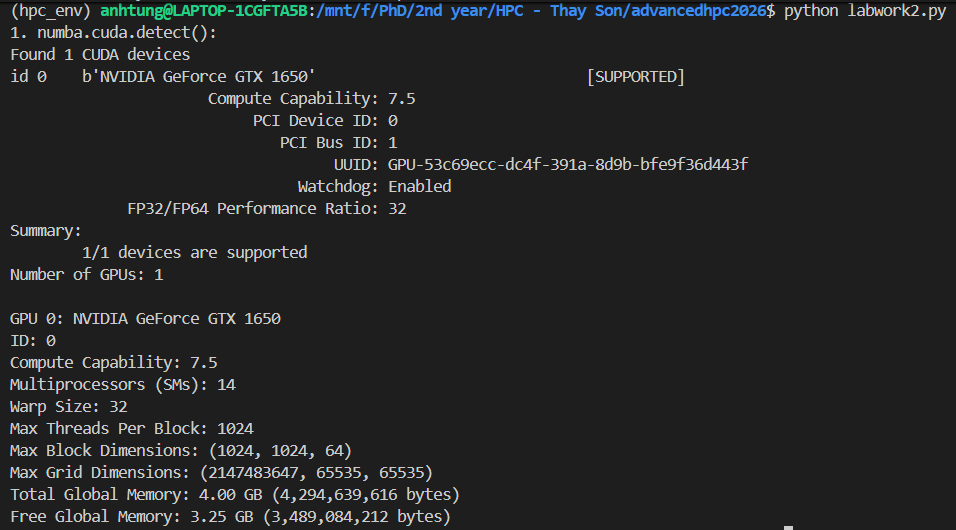
\includegraphics[width=0.9\textwidth]{output.png}
    \caption{Console output of the GPU hardware inspection.}
    \label{fig:gpu_output}
\end{figure}

\section{Brief Discussion}
\begin{itemize}
    \item The detected GPU provides sufficient compute capability and execution units to support SIMT parallel workflows in upcoming lab assignments.
    \item Parameters such as the warp size (32 threads) and maximum threads per block (1024) serve as architectural constraints for configuring grid and block dimensions in kernel launches.
\end{itemize}

\end{document}